\documentclass[sigconf,screen]{acmart}
% Camera-ready for the AgenticDev 2026 Workshop, built against the
% ACM Primary Article Template (acmart v2.20). The submitted version used
% [sigconf,nonacm]; ACM publication metadata is enabled here.
\usepackage{booktabs}
\usepackage{pifont}   % \ding{51}: Linux Libertine has no U+2713
\usepackage{float}   % [H]: pin the overview table in place
\usepackage{array}   % >{\raggedright\arraybackslash}p{} columns

% ---------------------------------------------------------------------------
% ACM PUBLICATION METADATA -- AUTHOR INPUT REQUIRED BEFORE SUBMISSION.
% The values below MUST be replaced with the ones ACM sends in the eRights
% confirmation email (rights statement, copyright year, DOI, ISBN). They are
% deliberately left as \acmXXX placeholders rather than invented: submitting
% fabricated rights metadata is worse than submitting none. Until eRights
% arrives, this file will typeset ACM's default "manuscript" rights block.
% ---------------------------------------------------------------------------
\acmConference[AgenticDev 2026]{International Workshop on Agentic AI for
Next-Generation Software Development}{October 12, 2026}{Munich, Germany}
\acmYear{2026}
% \setcopyright{rightsretained}      % <- from eRights email
% \acmDOI{10.1145/XXXXXXX.XXXXXXX}   % <- from eRights email
% \acmISBN{978-1-4503-XXXX-X/26/10}  % <- from eRights email

% Camera-ready typesetting: let TeX resolve the last few tight lines rather than
% letting them protrude into the margin.
\emergencystretch=1.5em
\Urlmuskip=0mu plus 1mu\relax   % let long URLs break across lines
\def\UrlBreaks{\do\/\do-\do.\do\_\do\&\do\=\do\?}
\hyphenation{re-pos-i-tory re-pos-i-to-ries lo-cal-i-za-tion ca-pa-bil-i-ty
in-her-i-tance con-straint-shar-ing pre-reg-is-tered in-fra-struc-ture
de-ter-min-is-ti-cally}

\newcommand{\ctx}{\texttt{context.md}}
\newcommand{\artifact}{\url{https://github.com/getmetatron/context-md}}
% ARTIFACT DOI -- AUTHOR INPUT REQUIRED. The replication package must be
% deposited in an archival repository (e.g. Zenodo/Software Heritage/figshare)
% and the resulting persistent DOI placed here. The GitHub URL above is a
% development link and is NOT an archival citation. Uncomment and fill:
% \newcommand{\artifactdoi}{\url{https://doi.org/10.5281/zenodo.XXXXXXX}}
\providecommand{\artifactdoi}{\textbf{[archival DOI pending deposit]}}

\begin{document}

\title{Context Inheritance: A Git-Native Architecture and Pre-Registered Study
of Repository Context for AI Coding Agents}

\author{Pavel Kerbel}
\authornote{Corresponding author. All authors are affiliated with Metatron Research (\url{https://getmetatron.com}); ORCIDs identify each author.}
\orcid{0009-0004-4679-1036}
\email{pavel@getmetatron.com}
\affiliation{\institution{Metatron Research}\city{Tel Aviv}\country{Israel}}
\author{Milana Kerbel}
\orcid{0009-0004-7893-9824}
\email{milana@getmetatron.com}
\affiliation{\institution{Metatron Research}\city{Tel Aviv}\country{Israel}}
\author{Vitali Abramov}
\orcid{0009-0007-0814-3822}
\email{vitali@getmetatron.com}
\affiliation{\institution{Metatron Research}\city{Tel Aviv}\country{Israel}}
\author{Liat Abramov}
\orcid{0009-0006-1601-146X}
\email{liat@getmetatron.com}
\affiliation{\institution{Metatron Research}\city{Tel Aviv}\country{Israel}}

\begin{abstract}
AI coding agents repeatedly rediscover project constraints, because repositories
version code but not operating knowledge: the decisions taken, the alternatives
rejected, the constraints found during execution. We introduce the
\emph{Repository Context Layer} (RCL)---the repository carries its own agent-facing
context, versioned with the code, deterministically discoverable, consulted by
contract, and writable by agents only under human review, in a minimal default
format, \ctx{}---and study, in a pre-registered experiment on SWE-bench Verified,
when it helps. The organizing observation is a \emph{capability-dependent
author--reader pattern} we call \emph{context inheritance}: repository context
behaves like senior knowledge, and across the levels we observe its value flows
toward weaker readers. A small local executor gains a large navigational benefit
from context authored by a more capable model (+26~pp localization on
topic-matched tasks, $p < 0.0001$) but nothing from context it wrote itself
($+0.0$~pp); with two author levels drawn from different model families, we
report this as a pattern consistent with a capability gradient rather than an
isolated causal variable. At the frontier the axes shift: an agent
appears to gain from its own failure-derived lessons, but not from answer-derived
ones (+14.6~pp resolve on constraint-sharing tasks; $p = 0.041$ uncorrected,
$0.081$ after Holm correction within its registered family, so we report the
direction rather than a confirmed effect; $-32\%$ tokens per resolved task); \emph{how}
context is delivered matters (exploratorily, a sharded store the agent reads
selectively outperformed a monolith at a third of the tokens at the local tier);
and on a broad
random sample a frontier agent sits at a resolve ceiling that no context improves.
The design consequence is concrete: version repository context as a first-class
artifact, author it with the strongest writer available, and expect the benefit in
cheaper agents that read it.
\end{abstract}

\begin{CCSXML}
<ccs2012>
<concept><concept_id>10011007.10011074</concept_id><concept_desc>Software and its engineering~Software creation and management</concept_desc><concept_significance>500</concept_significance></concept>
<concept><concept_id>10010147.10010178</concept_id><concept_desc>Computing methodologies~Artificial intelligence</concept_desc><concept_significance>300</concept_significance></concept>
</ccs2012>
\end{CCSXML}
\ccsdesc[500]{Software and its engineering~Software creation and management}
\ccsdesc[300]{Computing methodologies~Artificial intelligence}
\keywords{repository context, agentic software development, context.md, capability
gradient, context inheritance, agent memory, SWE-bench, pre-registered study}

\maketitle

\section{Introduction}
Coding agents crossed a practical threshold in 2024--2026: given a task, a modern
agent can plan, edit, run tests, and iterate over hours with little supervision.
What has not kept pace is the substrate those agents work on. A repository exposes
its code, but not the reasoning that produced the code. The result is a familiar
failure mode: an agent that writes competent code while re-proposing the library
the team removed, violating an unwritten layering rule, or re-discovering, at some
cost, a constraint a previous session had already found.

A concrete case: an agent reaches for an ORM to simplify a query, unaware the team
removed ORMs months earlier because query opacity had broken an offline repair
path. The decision lives in commit history and human memory---nowhere the agent
consults. It writes reasonable code that a reviewer must catch, or that ships and
regresses a constraint the project had already settled.

Practitioners mitigate this with a patchwork: instruction files
(\texttt{CLAUDE.md}, \texttt{AGENTS.md}, \texttt{.cursorrules}) inject standing
guidance; IDE memories persist preferences per tool; retrieval-augmented
generation (RAG)~\cite{lewis2020rag} recalls similar text; protocols such as
MCP~\cite{mcp2024} standardize access to external stores. Each helps; none yields
a durable, reviewable, project-owned operating context that improves as work
happens (Section~\ref{sec:background}).

This paper formalizes an alternative that requires no new infrastructure---the
repository carries its own operating context, versioned by Git, gated by code
review, and updated as a routine part of every change, a pattern we call the
\emph{Repository Context Layer} (RCL)---and then asks the question a practitioner
actually faces: \emph{given} such a layer, when does an agent benefit from it? The
answer is not uniform, and its structure is the paper's central finding.

\emph{Context inheritance.} We observe that the benefit an agent draws from
repository context tracks the capability of whoever \emph{wrote} the context
relative to the agent that \emph{reads} it. Context from a stronger author lifts a
weaker reader decisively; a self-taught weak model gains nothing; generic context
adds no broad-sample resolve gain to a frontier reader at ceiling, yet
failure-derived context cuts its constraint-sharing token cost by 32\%. Repository context
behaves like senior engineering knowledge whose value flows toward cheaper agents
that later read the repository. We call this pattern \emph{context inheritance}. We
observe two author levels drawn from different model families, so the experiment
does not isolate capability as the sole causal variable; what it establishes is a
consistent author--reader dependence, and that dependence reframes the practical
questions of who should author a context layer, who benefits, and when it is worth
the tokens.

\emph{Contributions.}
\begin{enumerate}
\item \textbf{The architecture.} A definition of the Repository Context Layer, its
six required properties, a Git-native lifecycle with branch/merge/rollback
semantics, a deterministic discovery specification, and a minimal file format
(Sections~\ref{sec:rcl}--\ref{sec:design}).
\item \textbf{Context inheritance: a capability-dependent author--reader pattern.}
Holding a small executor fixed, a blind frontier-authored seed raises localization
$+26.1$~pp ($p < 0.0001$) on topic-matched tasks while the executor's own lessons
move it $+0.0$~pp ($p = 1.0$). What transfers appears to depend on the reader:
directionally, a frontier agent draws on failure-derived lessons rather than the
answer-derived ones that serve the weak tier---a suggestive contrast that does not
clear correction for multiple comparisons
(Sections~\ref{sec:gradient}--\ref{sec:frontier}).
\item \textbf{When inheritance pays, and what it costs.} Delivery matters---a
sharded store the agent reads selectively outperformed a monolith at a third of
the context tokens, an exploratory contrast (Section~\ref{sec:delivery})---but inheritance has a ceiling: on a
broad random sample a frontier agent resolves 91\% of well-specified bugs unaided
and no delivery improves on it (Section~\ref{sec:ceiling}). Where it does pay it
is self-financing, at $-32\%$ tokens per resolved task (Section~\ref{sec:tokens}).
\end{enumerate}

We keep four concerns separate, because they can be adopted independently: the
\emph{architecture} (what the layer is), the \emph{discovery specification} (how
agents find it), the \emph{file format} (the default representation), and
\emph{implementations} (tools that automate it). A team can conform with nothing
but a Markdown file and a code-review habit.

\section{Background}\label{sec:background}
We survey the mechanisms teams currently use to convey project knowledge to
agents, against five properties the problem demands: persistence across sessions,
co-versioning with the code, agent writability, human review of changes, and
consultation by contract (the agent is required to read it, rather than hoping
retrieval surfaces it).

\emph{READMEs and documentation.} Durable and versioned, but usage-oriented: they
explain how to build and run, rarely why the architecture is shaped as it is, and
almost never what was rejected. Documentation also drifts, because nothing in the
workflow forces an update when a decision is reversed.

\emph{Architecture decision records.} ADRs~\cite{nygard2011adr} are the closest
ancestor of this work. They capture context, decision, and consequences, and they
live in the repository. But ADRs are write-once records addressed to future
humans. There is no contract obliging an agent to read them, no convention for
machine consumption, and no channel for an agent to contribute what execution
taught it. In practice ADR directories are archives, not operating context.

\emph{Wikis and design documents.} Detached from the repository, unversioned with
the code, and notorious for rot. A wiki page cannot branch with an experiment or
roll back with a revert.

\emph{RAG over project artifacts.} Retrieval by embedding
similarity~\cite{lewis2020rag} answers ``what text resembles this query,'' which
is the wrong question for constraints. A prohibition matters most precisely when
nothing in the current prompt resembles it; an agent adding a dependency will not
emit a query similar to the paragraph explaining why dependencies are frozen. RAG
also adds infrastructure, and its store is not reviewable by diff.

\emph{Agent memory systems.} A rich research line gives agents persistent memory:
Reflexion~\cite{shinn2023reflexion} stores verbal self-reflections on failures and
improves within a task series; Voyager~\cite{wang2023voyager} accumulates an
ever-growing library of validated skills; MemGPT~\cite{packer2023memgpt} pages
long-term memory in and out of the context window; generative
agents~\cite{park2023generative} maintain retrieval-scored memory streams. These
systems demonstrate that experience-derived memory improves agent
performance---the premise our evaluation revisits in a software-engineering
setting---but their stores are agent- or platform-owned: unversioned with any
codebase, invisible to code review, and not shared across heterogeneous tools
working on the same project. RCL relocates exactly this memory into the
repository's own trust machinery: the store branches, merges, and reverts with the
code, and every write passes human review. Our results add a boundary condition
this literature has not measured: the value of self-derived memory depends sharply
on the capability of the agent writing it (Section~\ref{sec:eval}).

\emph{IDE and platform memories.} Convenient and automatic, but scoped to one tool
and often one machine, invisible to teammates, and unreviewed. Two agents working
the same repository through different tools share nothing.

\emph{Agent instruction files.} \texttt{CLAUDE.md}, \texttt{AGENTS.md},
\texttt{.cursorrules}, and similar files are versioned, reviewed, and consulted by
contract, which is why they spread quickly. Their limitation is directionality:
they carry orders from the human downward, with no defined way to absorb what the
agent itself learns. They are static configuration, not evolving context.

\emph{Protocols.} MCP~\cite{mcp2024} and similar protocols standardize transport
between agents and external systems. Transport is orthogonal to persistence: a
protocol can serve a context layer, but does not itself provide one.

\begin{table}[t]
\caption{Project-knowledge mechanisms against the properties persistent agent
context requires.}
\label{tab:mechanisms}
\small
\begin{tabular}{@{}lcccc@{}}
\toprule
Mechanism & \shortstack{Versioned\\w/ code} & \shortstack{Agent-\\writable} & \shortstack{Human-\\reviewed} & \shortstack{Consulted\\by contract}\\
\midrule
README / docs & \ding{51} & --- & \ding{51} & ---\\
ADRs & \ding{51} & --- & \ding{51} & ---\\
Wiki / design docs & --- & --- & --- & ---\\
RAG store & --- & partial & --- & ---\\
IDE memories & --- & \ding{51} & --- & ---\\
Agent memory systems & --- & \ding{51} & --- & partial\\
Instruction files & \ding{51} & --- & \ding{51} & \ding{51}\\
\textbf{Context layer} & \ding{51} & \ding{51} & \ding{51} & \ding{51}\\
\bottomrule
\end{tabular}
\end{table}

The pattern in Table~\ref{tab:mechanisms} is the thesis of this section: each
mechanism solves a slice, and the missing artifact is the one with all four
properties at once.

\section{The Repository Context Layer}\label{sec:rcl}
A Repository Context Layer is a version-controlled, human-readable context store
that lives alongside the codebase and serves as the authoritative operating
context for AI agents working in it. The distinction from adjacent artifacts is
one of question: code captures what a system does; documentation explains how to
use it; the context layer records \emph{why} future changes should or should not
be made---the intent behind the design and the constraints that must survive it.

\begin{figure*}[t]
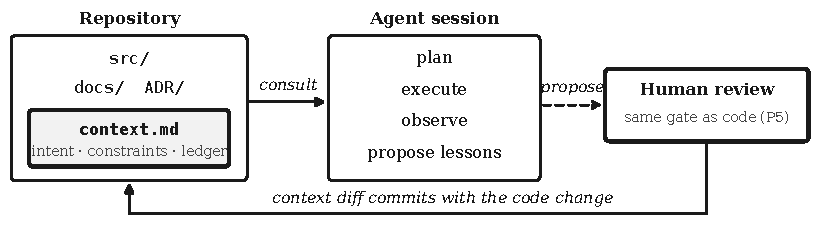
\includegraphics[width=\linewidth]{figures/fig1-architecture.pdf}
\Description{Block diagram. A Repository box containing src/, docs/ and ADR/, and a highlighted context.md holding intent, constraints and a ledger. An arrow labelled consult runs from the repository to an Agent session box listing plan, execute, observe and propose lessons. A dashed arrow labelled propose runs from the agent session to a Human review box annotated same gate as code (P5). A return path from human review back to the repository is labelled context diff commits with the code change.}
\caption{The Repository Context Layer is added alongside a repository's existing
artifacts. An agent consults it before planning and proposes updates after
executing; every update travels through the same review as the code that
motivated it.}
\label{fig:arch}
\end{figure*}

\subsection{Required properties}
An implementation conforms to the architecture if it satisfies six properties.
\textbf{P1 Co-versioned:} the context is stored in the repository and follows its
branching model. \textbf{P2 Human-readable:} the representation is plain text a
maintainer can read and edit without tooling. \textbf{P3 Deterministically
discoverable:} an agent locates the context by a fixed rule, not by search
(Section~\ref{sec:discovery}). \textbf{P4 Bidirectional:} agents both consume the
context and propose additions to it. \textbf{P5 Review-gated:} no change to the
context takes effect without passing the project's normal review process.
\textbf{P6 Tool-independent:} participation requires only the ability to read and
write files.

\subsection{Goals and non-goals}
The layer aims to hold the \emph{operating} knowledge of a project: intent,
binding constraints with their reasons, and validated lessons from execution. It
is deliberately not a knowledge base of the code itself (the code is present and
searchable), not a replacement for retrieval over large corpora, not a record of
conversations, and not a configuration system. A useful test: an entry belongs in
the layer if a competent new engineer would need to be told it, and would not
discover it by reading the code.

\subsection{Relationship to Git}
The architecture makes one load-bearing choice: it defines conventions over plain
files in Git rather than a new store. This buys provenance (\texttt{git blame}
answers who believed what, and when), review (the pull request is the approval
mechanism), branching and rollback (Section~\ref{sec:lifecycle}), distributed
synchronization, and audit, all without new infrastructure. The cost is Git's
limitations, notably textual rather than semantic merging;
Section~\ref{sec:design} discusses the consequences.

\subsection{Four layers}
We separate the pattern into independently adoptable layers: \textbf{L1}, the
architecture of this section; \textbf{L2}, the discovery specification of
Section~\ref{sec:discovery}; \textbf{L3}, the \ctx{} file format of
Section~\ref{sec:format}; and \textbf{L4}, implementations that automate
consultation, capture, and retrieval. A team may adopt L1--L3 with no tooling at
all; a vendor may implement L1--L2 with a different representation than L3.
Conformance claims should name the layers they cover.

\section{The Context Lifecycle}\label{sec:lifecycle}
The lifecycle is the behavioral half of the architecture: it defines when the
context is read and when it is written: \emph{consult} $\rightarrow$ \emph{plan}
$\rightarrow$ \emph{execute} $\rightarrow$ \emph{observe} $\rightarrow$
\emph{update} $\rightarrow$ \emph{review} $\rightarrow$ \emph{commit}.

\emph{Consult.} Before planning, the agent reads the context in full. Constraints
bind the plan; intent breaks ties among admissible designs. \emph{Plan /
Execute.} Ordinary agent operation. \emph{Observe.} On completion, the agent asks
what the work taught that a future session would otherwise re-learn. Most
observations are discarded; durability is the filter. \emph{Update.} Surviving
observations are appended to the context's ledger. \emph{Review.} The context diff
rides in the same change set as the code, and a human approves both together.
\emph{Commit.} The repository's knowledge and behavior advance atomically.

Four invariants summarize the contract. \textbf{I1:} consultation precedes
planning. \textbf{I2:} ledger writes are appends. \textbf{I3:} no context change
takes effect without review. \textbf{I4:} context changes travel with the code
changes that motivated them.

\emph{Branch behavior.} Because the context is a file, it branches when the code
branches. A learning made on an experimental branch is visible only there, which
is correct: it may be true only there. Deleting an abandoned branch deletes
beliefs that were never validated. \emph{Merge behavior.} Merging a branch merges
its context. Appends to a ledger from different branches usually touch different
lines and merge cleanly; a union merge strategy makes this explicit. Conflicting
edits to a constraint are semantic conflicts, and the architecture deliberately
routes them to a human: two branches that learned incompatible things have
surfaced a real disagreement. \emph{Rollback.} Reverting a commit reverts the
beliefs recorded in it. This is a feature: if the change that motivated a learning
is withdrawn, the learning's justification is withdrawn with it.

\section{Context Discovery Specification}\label{sec:discovery}
Discovery must be deterministic (P3): a fixed path is an API, and an agent must not
depend on search or inference to find its own operating contract. The key words
MUST, SHOULD, and MAY follow RFC~2119~\cite{rfc2119}. An agent MUST check
\texttt{.repo/context.md}, then \ctx{} at the repository root, and use the first
file found. The paths \texttt{.repo/context/} and \texttt{context/} (repository
root) are RESERVED for sharding of large contexts. Agents encountering either
before they support sharding MUST still honor the first rule; a repository that
shards SHOULD keep a root context file as the discoverable index into the shards.
Agents MUST ignore sections they do not understand and MUST NOT fail on additional
files or metadata.

\section{The Context File Format}\label{sec:format}
The default representation (L3) is a single CommonMark file with a top-level
\texttt{\#~Repository Context} heading and three required sections, in any order.
\emph{Intent} states what the project is and the design philosophy subordinate
decisions must serve; it is the tiebreaker among admissible designs.
\emph{Constraints} are the binding rules; each entry SHOULD carry its reason,
including what was rejected and why. Constraints are edited, not appended.
\emph{Evolved Context} is an append-only ledger of dated entries recording what
agents and humans learned during execution. Entries are never rewritten;
corrections are recorded as superseding entries. Entries that prove durable are
\emph{promoted}: moved into Constraints in a reviewed change.

\noindent{\scriptsize\emph{Illustrative ORM \ctx{} (not an experimental seed):}}\par
\vspace{1pt}
\noindent\fbox{%
\begin{minipage}{0.95\columnwidth}
\scriptsize\ttfamily
\# Repository Context\\
\#\# Intent\\
Local-first CLI; preserve offline repairability.\\
\#\# Constraints\\
- No ORM: opacity broke offline repair; use raw SQL only.\\
\#\# Evolved Context\\
- [2026-06-29] pkg x >=3 breaks ARM64; pin 2.3.x.
\end{minipage}}
\vspace{1pt}

Existing projects rarely start empty. A practical seeding procedure: distill each
ADR's decision and consequences into one Constraints entry; move durable guidance
out of instruction files; and start the ledger empty. Seeding is a single reviewed
commit.

\section{Design Discussion}\label{sec:design}
Five design choices attract consistent pushback; we record the reasoning.

\emph{One file or many.} One file is the default because the context is a working
set, not an archive: its purpose is to be read, in full, at the start of every
session. When a context genuinely outgrows one file, the reserved directories
admit sharding by topic, with the root file retained as the discoverable index.
The failure mode to resist is archival creep: a context file that tries to be
documentation stops being read.

\emph{Scope of append-only.} Append-only applies to the ledger, not the
layer. The ledger is an evidence log; rewriting evidence destroys the provenance
that makes it trustworthy. Constraints, by contrast, are current law and are
edited in place, with Git history preserving every prior state.

\emph{Merge conflicts.} Textual conflicts concentrate in the ledger, where
concurrent appends collide at the file's tail. Declaring a union merge for the
context file resolves concurrent appends automatically while leaving edits to
shared lines for humans. The architecture automates the merges that cannot be
wrong and refuses to automate the ones that can.

\emph{Hierarchical context.} Monorepos want scoped context. The v0.x position is
to standardize the root and defer hierarchy, reserving nearest-ancestor discovery
as the intended extension. Hierarchy multiplies the spec surface, and the pattern
should earn complexity with adoption evidence first.

\emph{Agent write authority and the threat model.} An agent may propose anything
and enact nothing. Every context change lands through the same review gate as code
(I3), so the ceiling on agent authority equals the rigor of the project's review
process. The gate is also the security boundary: a context layer is standing
instruction to future agents, making a poisoned entry persistent prompt injection.
Three properties contain this: review-gating (P5) means hostile entries must pass a
human; provenance (P1) means every entry has an author, a commit, and a motivating
change; human-readability (P2) denies attackers obscurity. Reviewers SHOULD treat
context diffs with the scrutiny of code diffs, and conformant tooling MUST refuse
to promote files that do not explicitly declare themselves context documents. The
gate must also scale: an agent attempting dozens of tasks a day would exhaust
reviewer attention if every raw lesson demanded fresh scrutiny. Automated
pre-screening therefore belongs in front of the human---format and size linting,
classifiers that flag privilege-expanding or outward-pointing instructions, and
mechanical promotion rules such as the rubric our evaluation uses---so the reviewer
sees few, well-formed, pre-vetted diffs rather than a stream of candidates. In our
evaluation such a rubric screened every candidate lesson with no human in the loop,
rejecting roughly one in ten before review---chiefly entries too narrow to be
repository-general (naming a specific instance or line number) and, less often,
over-length entries failing the size lint.

\section{What the Layer Is Not}
It is not RAG: consultation is by contract, not similarity. It is not prompt
engineering: instruction files configure behavior top-down and are static between
human edits, while the layer evolves through execution. It is not documentation:
docs address human onboarding at human timescales; the layer is machine-facing
operating state. And it is not chat memory: platform memories attach to a user or
a tool, while repository context attaches to the artifact all users and tools
share. The distinctions matter because each framing suggests the wrong lifecycle:
archives are allowed to go stale, and this must not.

\section{Reference Implementation}\label{sec:impl}
A reference implementation, Metatron~\cite{metatron}, implements all four layers
(L1--L4) for teams that want the lifecycle automated: project knowledge as
individual Markdown files in an open knowledge format, one decision per file with
structured front matter, sharded under a root-level \texttt{context/} directory,
with a scaffolded root \ctx{} whose Constraints point into the shards---so
discovery works for any conformant agent with no tool-specific knowledge. Candidate
entries flow through an explicit review step before becoming canonical. The
implementation exists to reduce friction, not to be required: a team using plain
\ctx{} with disciplined review conforms to the same architecture.

Current agents need a one-time bootstrap telling them the contract exists; the
natural place is the instruction file they already read (\texttt{CLAUDE.md},
\texttt{AGENTS.md}, \texttt{.cursorrules}, or a system-prompt sentence). This
yields a clean division of labor: the instruction file tells the agent that the
context layer exists; the context layer holds what the agent needs to know.
Because every integration reads the same artifact, a repository worked on by three
different tools accumulates one shared context rather than three private memories.

\section{Empirical Evaluation}\label{sec:eval}
We evaluate the architecture's central behavioral claims---that repository-carried
context measurably changes agent behavior, and that its benefit is
capability-dependent---in a pre-registered experiment on SWE-bench
Verified~\cite{swebench,swebenchverified}. The protocol (hypotheses, conditions, metrics, analysis
plan, power simulation) was frozen and externally timestamped at a git tag before
any confirmatory run; pilots are excluded. The released materials include the
frozen protocol, blind-authoring audit record, completed-episode transcripts,
runner-failure records, promotion logs, and containerized evaluation
verdicts~\cite{artifact}.

\subsection{Design}
\emph{Transfer pairs.} SWE-bench Verified supplies real historical bugs, each with
a hidden grading suite and the maintainers' fix (the \emph{gold patch}). We
identified \emph{constraint groups}---instances within one repository whose fixes
depend on the same convention (e.g., xarray's \texttt{keep\_attrs} propagation;
Django's \texttt{deconstruct()} fidelity rules)---and froze ordered transfer pairs
$(A,B)$ before any run: $B$ is held out, and the treatment's only advantage on $B$
is context derived from working on $A$. This constraint-sharing regime is about
8\% of the benchmark---the setting the architecture is designed for---and we also
evaluate a broad random sample (Section~\ref{sec:ceiling}).

\emph{Conditions.} Executors: a frontier model (Claude Opus 4.8) and a small local
model (Gemma~4, 8B, Q4\_K\_M quantized), in an identical minimal scaffold; every episode is
a fresh session in a freshly cloned checkout, no state carried across episodes.
Context authors: none; the executor itself (self-authored, via the lifecycle); a
more capable model given only a years-old, history-stripped checkout and
constraint-group names, never a problem statement, patch, or test (a blind seed);
or a labeled oracle bound shown the gold patch (never pooled). \textbf{No context
was produced by an automatic extraction pipeline}: all authored context is blind-
or lifecycle-derived by design, isolating the context-author condition while
holding the executor and delivery setup fixed, and limiting solution leakage
(audited in Section~\ref{sec:threats}). Delivery: injected into
the prompt, a monolithic \ctx{}, or a sharded store read selectively under a
consultation contract. Metrics: consultation, gold-file localization, resolve
(official containers), and tokens. Paired comparisons use sign-flip permutation
tests (10k draws, fixed seed); families are Holm-corrected.

Table~\ref{tab:design} states the full matrix once; every result section below is
one row of it. Two task sets recur and should not be conflated: the
\emph{topic-matched} set (the 36 frozen transfer pairs, where held-out task $B$
shares a constraint with $A$) and the \emph{broad} sets (a 267-instance pool and
an 88-instance random sample, neither selected for shared constraints). The
architecture targets the first; the second bounds what it is worth elsewhere.



\begin{table}[H]
\caption{The complete experimental matrix. Each results section varies one axis
and holds the rest fixed. ``Frontier seed'' was authored from a history-stripped
checkout and constraint-group names only; ``oracle'' arms were shown the gold
patch of the \emph{source} task $A$ and are never pooled with confirmatory arms.
\emph{Matched} task sets are the frozen transfer pairs, in which the held-out task
shares a constraint with the source task; \emph{broad} and \emph{random} sets are
not selected for shared constraints.}
\label{tab:design}
\footnotesize
\setlength{\tabcolsep}{3.5pt}
\begin{tabular}{@{}l>{\raggedright\arraybackslash}p{0.20\linewidth}>{\raggedright\arraybackslash}p{0.36\linewidth}>{\raggedright\arraybackslash}p{0.22\linewidth}@{}}
\toprule
\S & Executor, metric & What varies & Task set (ep./arm)\\
\midrule
\ref{sec:gradient} & 8B, localization & author: none, blind frontier seed, oracle bound & 36 matched (180)\\
\ref{sec:gradient} & 8B, localization & author: self (condition D lifecycle) & 12 matched (60)\\
\ref{sec:frontier} & frontier, resolve & author: none, self (failure), oracle (answer) & 16 matched (48)\\
\ref{sec:delivery} & 8B, localization & delivery: none, inject, file, shard & 267 broad (801)\\
\ref{sec:ceiling} & frontier, resolve & delivery: none, inject, file, shard & 88 random (88)\\
\ref{sec:tokens} & frontier, tokens & author: none, self (failure), oracle & 16 matched (48)\\
\bottomrule
\end{tabular}
\end{table}

\subsection{Context from a stronger author benefits the local executor}\label{sec:gradient}
Holding the executor fixed at 8B (36 pairs $\times$ 5 repetitions = 180 held-out
episodes per arm), the held-out outcome varies only with who authored the context
(Figure~\ref{fig:gradient}). A blind frontier-authored seed raises gold-file
localization from 21.1\% to 47.2\%---$+26.1$~pp, $p < 0.0001$---and a gold-distilled
bound to 42.8\% ($+21.7$~pp, $p < 0.0001$); the two capable-author tiers are
statistically indistinguishable. The executor's \emph{own} promoted lessons---162
across 60 pair-repetitions---move localization by $+0.0$~pp ($p = 1.0$): exactly the
no-context control. In this experiment, then, context from either capable author
approximately doubled the 8B executor's localization relative to no context, while
its self-authored lessons produced no measurable localization improvement. We
observe two author levels only, so we cannot distinguish a threshold from a steep
dose curve; author and executor also come from different model families, so author
capability and family characteristics are not separated here. A within-family
author-size sweep would settle both; we did not run one. The 8B model used
frontier-written context effectively, but its own lessons did not improve
localization under this setup: it recorded tooling tactics rather than the
repository constraints the frontier author captured under the identical prompt. At this tier the movement
is in localization, not resolve (all arms 5--8\%; pooled oracle $+2.2$~pp,
$p = 0.22$).

\begin{figure}[t]
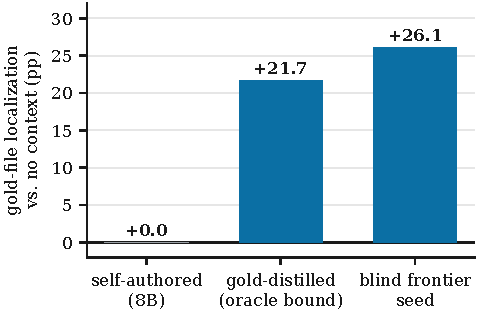
\includegraphics[width=\linewidth]{figures/fig3-gradient.pdf}
\Description{Bar chart of paired change in the 8B executor's gold-file localization relative to its no-context control, by who authored the context. Self-authored context is at plus 0.0 percentage points, a gold-distilled oracle bound at plus 21.7, and a blind frontier-authored seed at plus 26.1.}
\caption{Paired improvement in the 8B executor's gold-file localization over its
no-context control, by context author (36 pairs $\times$ 5 repetitions). Both
capable-author conditions approximately doubled localization here; the executor's
self-authored context sat on the no-context floor. Resolve deltas are not
significant at this tier.}
\label{fig:gradient}
\end{figure}

\subsection{At the frontier, the transfer pattern differs}\label{sec:frontier}
Running the full lifecycle with the frontier executor on 16 constraint-sharing
pairs ($\times$ 3 repetitions, 48 held-out episodes/arm), the agent's own
failure-derived lessons---extracted from working task $A$, never seeing a gold
patch or hidden test---raise held-out resolve on $B$ from 58.3\% to \textbf{72.9\%}
($+14.6$~pp; localization $91.7$ vs.\ $81.2\%$; of the 11 constraint groups 7
improve, 3 are flat, and 1 declines; Figure~\ref{fig:slope}). These are uncorrected paired permutation $p$-values
($0.041$ and $0.064$); Holm correction across the two contrasts in this registered
family puts both at $0.081$, so the effect does not clear the pre-registered bar
and we report its direction rather than a confirmed difference. The correction
changes the \emph{inference}, not the estimate: the effect size remains
$+14.6$~pp; what changes is that, once the family is accounted for, this sample
does not license calling it established. H2 (treatment over
control on held-out $B$) was pre-registered; the \emph{inversion} reading below---that
what transfers switches from answers to failures as the reader gets stronger---was
not a registered hypothesis and is post hoc. Yet lessons distilled from the
\emph{gold patch} transfer nothing at this tier (60.4\% resolve, indistinguishable
from no context). The observed pattern is directionally opposite to the weak tier,
where gold-distilled
context was the strongest author: answer-derived lessons encode solutions;
failure-derived lessons encode traps and process. A weak reader needs to be told
where things are; a strong reader already localizes and needs to be told where it
will go wrong. What is inherited depends on the reader.

\begin{figure}[t]
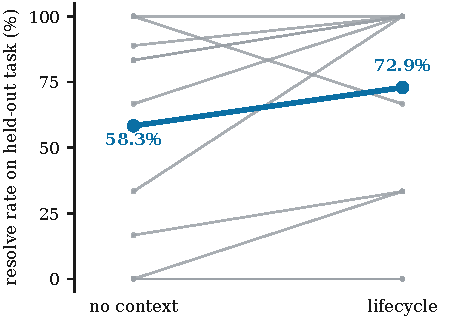
\includegraphics[width=\linewidth]{figures/fig2-slopegraph.pdf}
\Description{Slopegraph of frontier-executor resolve rate on held-out tasks, from the no-context arm on the left to the lifecycle arm on the right. Eleven grey lines show the constraint groups: seven rise, three are flat and one falls. A bold line shows the overall episode-level mean rising from 58.3 percent to 72.9 percent.}
\caption{Frontier executor resolve rate on held-out tasks, without and with the
lifecycle. Gray lines: the 11 constraint groups (7 improve, 3
are flat, 1 declines); the bold line is the overall episode-level mean. The
$+14.6$~pp difference is directional: $p = 0.041$ uncorrected, $0.081$ after Holm
correction within its registered family.}
\label{fig:slope}
\end{figure}

\subsection{Delivery shapes inheritance}\label{sec:delivery}
Holding content fixed (the blind seed) and varying only \emph{how} it is
delivered, we ran four conditions with the local executor on a frozen 267-instance
pool (3 repetitions, 801 episodes/arm): no context (B), injected (E), a monolithic
file (FILE), and a sharded store the agent reads selectively (SHARD). The
procedural consultation contract binds at scale---FILE and SHARD are consulted in
97\% of episodes, confirming the agent reliably reads the layer when instructed.
On the fixed 40-episode audit sample, author-confirmed labels agreed with the
detector on all three constructs (40/40 for consultation, deep read, and read
before edit; 38 positive and 2 negative; $\kappa=1.00$). This was an AI-assisted,
non-blinded verification, so we treat raw agreement as descriptive confirmation,
not as independent inter-rater reliability; with only two negatives, kappa is
also unstable.
The delivery mechanisms then separate (Table~\ref{tab:delivery}). SHARD is best on
localization (53.4\%) and, decisively, cheapest: it pays $\sim$3$\times$ fewer
context tokens than the monolith (305 vs.\ 902 per episode, $p = 0.0002$) because the
agent reads the index plus only the relevant shard(s), while FILE forces the whole
file through the transcript. The monolith is numerically \emph{below} the
no-context baseline on localization (46.8 vs.\ 48.6\%) while paying the most
tokens---plausibly crowding task reasoning in a bounded window. Under the
registered family (each mechanism against no-context and against injection, Holm
corrected), no single contrast clears the bar---SHARD$-$B is $+4.9$~pp, Holm
$p = 0.058$, a hair short---but the sharpest separation in the data is between the
two file mechanisms themselves. Exploratorily, selective sharding outperformed the
monolithic file by $+6.6$~pp ($p = 0.0007$) while using roughly one third of the
context tokens. These exploratory results suggest that selection can outperform
volume: making the agent \emph{choose} what to read both helped and cost less
here. If that reading holds, it extends the gradient's lesson from \emph{who
authored} the context to \emph{how much} of it is placed before the reader.

\begin{table}[t]
\caption{Local executor (8B), delivery of identical content. 801 episodes/arm.
Context tokens are the payload read into the transcript.}
\label{tab:delivery}
\small
\begin{tabular}{@{}lcccc@{}}
\toprule
delivery & localization & consulted & \shortstack{ctx tokens\\/episode} & resolve\\
\midrule
none (B) & 48.6\% & --- & 0 & 5.6\%\\
injected (E) & 51.2\% & --- & 930 & 8.6\%\\
file (FILE) & 46.8\% & 97\% & 902 & 7.0\%\\
sharded (SHARD) & \textbf{53.4\%} & 97\% & \textbf{305} & 6.7\%\\
\bottomrule
\end{tabular}
\end{table}

\subsection{Inheritance has a ceiling}\label{sec:ceiling}
The results above hold in the constraint-sharing regime the layer is built for.
Outside it, the picture changes. We ran all four delivery conditions with the frontier executor on an
88-instance stratified subset (one repetition; Figure~\ref{fig:ceiling}). The
no-context baseline already resolves \textbf{90.9\%} of these well-specified,
isolated bugs: the frontier model does not need repository context to fix bugs it
can already localize, and there is no headroom for context to add resolution. No
delivery beats the baseline; the small differences among B/E/FILE ($\pm$ a few
instances on $n=88$) are within noise. The contract still binds---FILE and SHARD
read the context in 100\% of episodes---so the null is not a failure to read; it
is that reading generic context on a random bug has nothing to contribute. Here
the selective store's economics also \emph{invert}: a capable model turns ``read
only what you need'' into thorough exploration, so SHARD spends 38.4K prompt tokens
against FILE's 24.0K and costs $\sim$50\% more per resolved task---the opposite of
the local tier, where SHARD was cheapest. Inheritance requires a reader below its
ceiling as well as an author above it; a frontier model on well-specified bugs
violates the first condition, and generic context becomes a cost, not a benefit.

\begin{figure}[t]
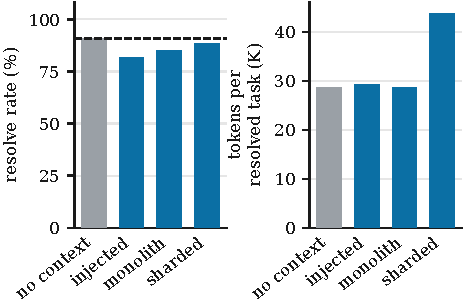
\includegraphics[width=\linewidth]{figures/fig5-ceiling.pdf}
\Description{Two bar charts for the frontier executor on an 88-instance random sample. Left: resolve rate by delivery mechanism, with no context at 90.9 percent marked by a dashed ceiling line, and injected, monolith and sharded delivery all below it. Right: tokens per resolved task, where the sharded store costs about 44 thousand against roughly 29 thousand for the other arms.}
\caption{Frontier executor on a broad 88-instance random sample: resolve rate by
delivery. No arm exceeds the no-context ceiling (dashed); the sharded store
recovers most but at the highest per-resolved cost. Costs are notional, at list
prices, excluding prompt caching.}
\label{fig:ceiling}
\end{figure}

\subsection{Where it pays, inheritance is self-financing}\label{sec:tokens}
In the constraint-sharing regime, the frontier lifecycle spends 55.7K tokens per
resolved task against 81.8K with no context ($-32\%$;
Figure~\ref{fig:tokens})---and the decomposition is telling: episodes ending in a
fix cost the same in both arms ($\approx$33.6K); the entire saving comes from
fewer doomed explorations. The oracle arm saves tokens identically without
converting them into resolves: context of either kind shortened wandering here,
but only the failure-derived condition also shows the directional resolve
improvement reported in Section~\ref{sec:frontier}. The local executor shows the
opposite sign ($+20\%$ tokens per episode with the seed): for a strong reader in
the right regime context is self-financing; for a weak one it is a paid
navigational upgrade. The frontier arms consumed a few hundred dollars of API spend,
consistent with the economic premise: expensive knowledge, written once, read
cheaply forever.

\begin{figure}[t]
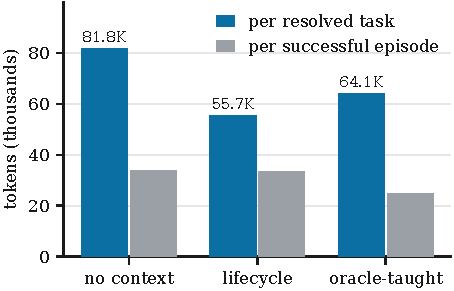
\includegraphics[width=\linewidth]{figures/fig4-tokens.pdf}
\Description{Grouped bar chart of token cost for the frontier executor in the constraint-sharing regime, comparing no context, the lifecycle and an oracle-taught arm. Tokens per resolved task fall from 81.8 thousand without context to 55.7 thousand with the lifecycle, while tokens per successful episode are close to 33.6 thousand in both.}
\caption{Tokens per resolved task (frontier executor, constraint-sharing regime).
Successful episodes cost the same in both arms; the saving comes from fewer failed
explorations. The oracle-taught variant spends like the lifecycle arm without
matching its resolve rate.}
\label{fig:tokens}
\end{figure}

\subsection{Threats to validity}\label{sec:threats}
\emph{Benchmark scope.} SWE-bench Verified supplies well-specified, isolated bug
fixes graded by hidden tests---a task type where localization is half the battle
and a frontier model already localizes almost unaided, which is precisely why the
ceiling (Section~\ref{sec:ceiling}) appears. It cannot measure a context layer's
central real-world value---adherence to conventions and avoidance of rejected
approaches---where ``correct'' is not ``tests pass.'' The frontier ceiling is thus
a statement about this task type, not about repository context in general: it is
in long-lived repositories carrying implicit architectural constraints, not in
isolated well-specified fixes, that a frontier reader would retain headroom for
context to lift. A benchmark scoring convention-adherence is the natural next
instrument. \emph{Extraction untested.} All authored context here is
blind- or lifecycle-derived, deliberately, to vary the author-capability contrast
and limit leakage; whether an automatic pipeline can \emph{produce} context of
comparable value is a separate question this design brackets, and the clearest
follow-up. \emph{Statistical scope.} The gradient (180 episodes/arm) and delivery
matrix (801/arm) are the robust core; the frontier resolve effect ($n=16\times3$)
and broad-sample matrix ($n=88\times1$) have wider intervals and are reported with
their caveats. Potential executor contamination affects both arms of within-model comparisons
symmetrically and would tend to compress deltas toward zero. Potential
contamination of the seed \emph{author} is not symmetric---it could favor the
treatment---and is considered separately in the leakage audit below. A local-tier resolve improvement
marginal in the initial pair set ($p = 0.066$) did not survive the pre-planned
expansion (pooled $p = 0.22$) and is not claimed; the frontier failure-vs-answers
contrast is marginal ($p = 0.067$) and reported as directional.

\emph{Blind-seed leakage audit.} The seed author never sees a problem statement,
patch, or test, but it does receive the repository and the constraint-group
names---and those names point at the convention under test, while these
repositories are almost certainly in the frontier author's pretraining. A seed that
partially distilled the answer would bias the treatment rather than cancel, so we
audited the seeds against the held-out gold patches (Table~\ref{tab:leakage}). The
seed names a file the fix edits for 83\% of held-out instances against 32\% for
same-repo instances it was never directed at, and a symbol the fix touches 56\%
versus 4\% of the time. This is strong evidence of topic and localization
conditioning: the seed reliably knows \emph{where} the relevant machinery lives,
which is unsurprising given that an experimenter chose the constraint groups it was
pointed at. Surface overlap with the fix itself is much weaker (identifier Jaccard
$0.019$ vs.\ $0.013$ on the same seed text, which holds length fixed), which is
some evidence against literal reproduction of patch content. Two limits should be
read with these numbers. First, the audit measures textual overlap, so it cannot
rule out partial solution knowledge mediated by pretraining and expressed in
different words. Second, it is an observational audit, not a manipulation. Taken
together the results are \emph{consistent with} a primarily navigational effect,
and the delivery experiment points the same way---the identical seed is worth
$+26.1$~pp on topic-matched pairs but $+4.9$~pp on the broad 267-instance pool
(Section~\ref{sec:delivery})---but they do not settle the contamination question.
We therefore treat the $+26.1$~pp figure as explicitly conditional on
experimenter-selected topic match, and $+4.9$~pp as the more task-agnostic
estimate. Analysis code and per-instance scores are released with the
artifact~\cite{artifact}.

\begin{table}[t]
\caption{Overlap between the blind seed and the gold patch of the instance the
executor was held out on, against the same seed text scored on same-repo instances
outside the study set. Holding the seed fixed across both columns controls for
length.}
\label{tab:leakage}
\small
\begin{tabular}{@{}lcc@{}}
\toprule
Seed overlap with the gold patch & held-out $B$ & non-study \\
 & ($n=36$) & ($n=257$) \\
\midrule
names a file the fix edits & 83.3\% & 32.3\% \\
names a symbol the fix touches & 55.6\% & 3.9\% \\
identifier Jaccard with the patch & 0.019 & 0.013 \\
\bottomrule
\end{tabular}
\end{table}

\emph{Deviations from the frozen protocol.} The full log is released with the
artifact; the material items are these. (i)~The registered analysis plan names
mixed-effects logistic regression and McNemar, whereas the reported tests are
paired sign-flip permutation tests; the protocol was internally inconsistent, and
the implementation followed the section whose power simulation was itself built
on the permutation test. (ii)~The registered local-tier constraint-violation
metric was \emph{never implemented}, so of the two local primaries only
wrong-file-edit rate was collected --- the metric closest to the architecture's
convention-adherence claim is missing. (iii)~The frontier tier ran 16 pairs
against a registered target of at least 25, which is a direct cause of the wide
interval on the frontier effect. (iv)~Registered conditions F (locally authored
seed) and G (human-authored seed) and research question RQ3 (accumulation across
a sequence) were not run. Consequently the self-authored arm reported here is
condition~D, the emergent lifecycle, and is \emph{not} the registered condition~F
self-authored seed; the two are different treatments. (v)~The delivery study's
protocol was frozen in a private repository, so its pre-registration provenance
is weaker than the main study's, which is publicly verifiable at an annotated tag.
(vi)~Two of 48 planned frontier no-context attempts terminated before producing
episode records. They remain in the planned denominator and are scored unresolved;
the released batch log records both nonzero runner outcomes.

\emph{Specification scope versus evidence scope.} The normative half of this paper
is broader than the experiment. The study exercises discovery
(Section~\ref{sec:discovery}), the consultation contract (consulted in 97--100\% of
episodes), the lesson lifecycle (Section~\ref{sec:lifecycle}), and the file format.
It does \emph{not} measure the review gate's usefulness, branch/merge/rollback
behavior under concurrent edits, or containment of a poisoned entry; those clauses
are proposed convention, justified by analogy to code review rather than by
evidence here, and should be read as such.

\section{Discussion and Future Work}
The results carry three practical consequences. Authorship should go to the most
capable writer available---a human expert, a frontier model, or distillation from
authoritative fixes---rather than to the working agents themselves, whose
self-authored context did not help them here. The beneficiaries are those cheaper agents: one authoring
pass, paid once, propagates navigational knowledge to every agent that later reads
the repository at zero marginal inference cost. And the layer earns its tokens only
where the reader sits below its ceiling and the context matches the task at
hand---weaker models broadly, stronger models on work that is ambiguous,
convention-laden, or re-hits a known constraint.

\emph{Future work.} Several directions follow. \emph{Validation:} conformance
linting for the format and, more usefully, for the lifecycle---CI integrations
(e.g., a pull-request action producing semantic context-diff summaries) that flag
substantive code changes landing with no context diff over long periods.
\emph{Semantic merging:} LLM-assisted reconciliation of contradictory ledger
entries, proposed to a human rather than applied. \emph{Summarization and
budgets:} automatic distillation of aging ledgers so the working set stays small
enough to be read in full. \emph{Hierarchy:} the nearest-ancestor extension for
monorepos that want scoped context. \emph{Cross-repository inheritance:}
organization-wide constraint layers that member repositories extend---the
capability gradient suggests a single well-authored parent could lift many
child repositories at once. \emph{Beyond the benchmark:} SWE-bench measures
isolated bug-fix correctness; a benchmark that scores convention-adherence and the
avoidance of rejected approaches would probe the value the frontier ceiling hides.
And---most pointedly, given the extraction result this study deliberately
brackets---measuring whether an automatic extraction pipeline can author context
of frontier-blind quality, by varying the context's author (blind-frontier vs.\
machine-extracted vs.\ human-curated) with delivery and executor held fixed.

\section{Conclusion}
Software repositories version their code, tests, documentation, and
infrastructure; this paper argues, and measures, that they should also version
their operating context. The architecture asks for no new infrastructure, reuses
the trust machinery of Git and code review, and degrades to a single Markdown
file. Whether it helps appears to be less a property of the layer than of the
relation between its author and its reader---the same seed is transformative for a
small executor on matched work and inert for a frontier model on a random bug.
Within the levels we could observe, the practical reading is to author repository
context with the strongest writer available and to expect the benefit in cheaper
agents that read it.

\section*{Conflicts of Interest}
All authors are affiliated with Metatron Research, whose open-source
implementation of the repository-context pattern (Metatron) motivates this study.
The experiment mitigates this competing interest by pre-registration before data
collection, a scaffold-uniform minimal harness rather than the product itself,
context that is blind- or lifecycle-authored rather than produced by that
implementation, and fully public data and analysis code.

\section*{AI-Assisted Preparation Statement}
Consistent with COPE guidance, the authors disclose that large language models
(Anthropic Claude and OpenAI Codex) assisted with manuscript drafting, analysis
scripting, experiment orchestration, and preparation of row-level evidence for
the consultation detector verification under continuous author direction and
review. The author reviewed and confirmed all audit labels and takes full
responsibility for the final text and all reported results.

\section*{Data Availability Statement}
The empirical values reported in this paper can be recomputed from the replication
package~\cite{artifact}, prepared for archival at \artifactdoi. It contains the
main study's pre-registration frozen at a publicly verifiable tag before any
confirmatory run; the delivery-study protocol, whose weaker private-tag provenance
is disclosed above; the seed-authoring audit record (\texttt{seeds/AUDIT.md}),
which documents the blind-authoring procedure, inputs, and prohibitions; the
leakage audit; the complete harness; episode predictions, promotion decisions,
runner-failure records, containerized evaluation verdicts; the completed
consultation detector audit and author verification record; and the analysis
scripts. The audit's AI-assisted, non-blinded confirmation procedure is disclosed
with the artifact and as a protocol deviation. The development repository is
\artifact.

\begingroup\small\sloppy
\begin{thebibliography}{9}
\bibitem{manifesto} P.~Kerbel. ``The Repository Context Layer: The Missing Layer
of Agentic Software Development,'' manifesto and specification repository, 2026.
\url{https://github.com/kerbelp/repository-context-layer}.
\bibitem{lewis2020rag} Patrick Lewis, Ethan Perez, Aleksandra Piktus, et al. 2020.
Retrieval-Augmented Generation for Knowledge-Intensive NLP Tasks. In \emph{NeurIPS
33}.
\bibitem{mcp2024} Anthropic. 2024. Introducing the Model Context Protocol.
\url{https://modelcontextprotocol.io}.
\bibitem{nygard2011adr} Michael Nygard. 2011. Documenting Architecture Decisions.
\bibitem{rfc2119} Scott Bradner. 1997. Key Words for Use in RFCs to Indicate
Requirement Levels. IETF RFC 2119.
\bibitem{shinn2023reflexion} Noah Shinn, Federico Cassano, Ashwin Gopinath,
Karthik Narasimhan, and Shunyu Yao. 2023. Reflexion: Language Agents with Verbal
Reinforcement Learning. In \emph{NeurIPS 36}.
\bibitem{wang2023voyager} Guanzhi Wang, Yuqi Xie, Yunfan Jiang, et al. 2024.
Voyager: An Open-Ended Embodied Agent with Large Language Models. \emph{TMLR}.
arXiv:2305.16291.
\bibitem{packer2023memgpt} Charles Packer, Sarah Wooders, Kevin Lin, et al. 2023.
MemGPT: Towards LLMs as Operating Systems. arXiv:2310.08560.
\bibitem{park2023generative} Joon Sung Park, Joseph O'Brien, Carrie Jun Cai,
Meredith Ringel Morris, Percy Liang, and Michael S. Bernstein. 2023. Generative
Agents. In \emph{UIST '23}. ACM.
\bibitem{swebench} C.~E. Jimenez et al. 2024. SWE-bench: Can Language Models
Resolve Real-World GitHub Issues? In \emph{ICLR 2024}.
\bibitem{swebenchverified} OpenAI. 2024. Introducing SWE-bench Verified: a
human-validated subset of SWE-bench.
\url{https://openai.com/index/introducing-swe-bench-verified/}.
\bibitem{metatron} P.~Kerbel. ``Metatron: a files-first repository context layer
for AI coding agents,'' software, v0.12.0, 2026.
\url{https://github.com/kerbelp/metatron}.
\bibitem{artifact} P.~Kerbel, M.~Kerbel, V.~Abramov, and L.~Abramov. ``RCL
efficacy study: pre-registered protocol and replication artifacts,'' 2026.
\artifactdoi{} (development repository: \artifact).
\end{thebibliography}
\endgroup

\end{document}
